\chapter{Examining the Generalisability of Automatic Most Likely Catalogue Matching}\label{ch:SNNGeneralisation}

As outlined in Chapter \ref{ch:ID}, an automatic approach to most likely catalogue matching was developed through the use of Siamese Neural Networks (SNNs). This approach, when tested using the NDD AU SMRU dataset developed in Chapter \ref{ch:NDD}, yields high top-1, top-5, and top-10 accuracies. However, it is not yet clear if these results are to be expected regardless of the photo-id catalogue utilised, or if there is an underlying property inherent to the NDD AU SMRU dataset that makes it particularly susceptible to an SNN-based approach. In this Chapter, automatic most likely matching is performed on a second, previously unseen, photo-id catalogue, allowing for an evaluation of the approach's generalisability.

\section{The SDRP Dataset}\label{ch:SNNGeneralisation,sec:SDRPDataset}

To evaluate the SNN approach's generalisability, a subset of photo-id catalogue data was obtained from the Chicago Zoological Society's Sarasota Dolphin Research Program (SDRP). The subset consisted of 250 images of 23 individual common bottlenose dolphins captured in the waters around Naples, FL, USA \cite{tyson_moore_final_2020}. Unlike the datasets collected from fieldwork in Northumberland, UK, the SDRP dataset was provided in a pre-processed form as the dataset had been previously utilised to compare photo-id methodologies \cite{tyson_moore_rise_2022}. Images provided were cropped to remove a large amount of background noise and centre the dorsal fin, examples of which can be seen in Figure \ref{fig:sdrp-example}. 

\begin{figure}
	\begin{center}
		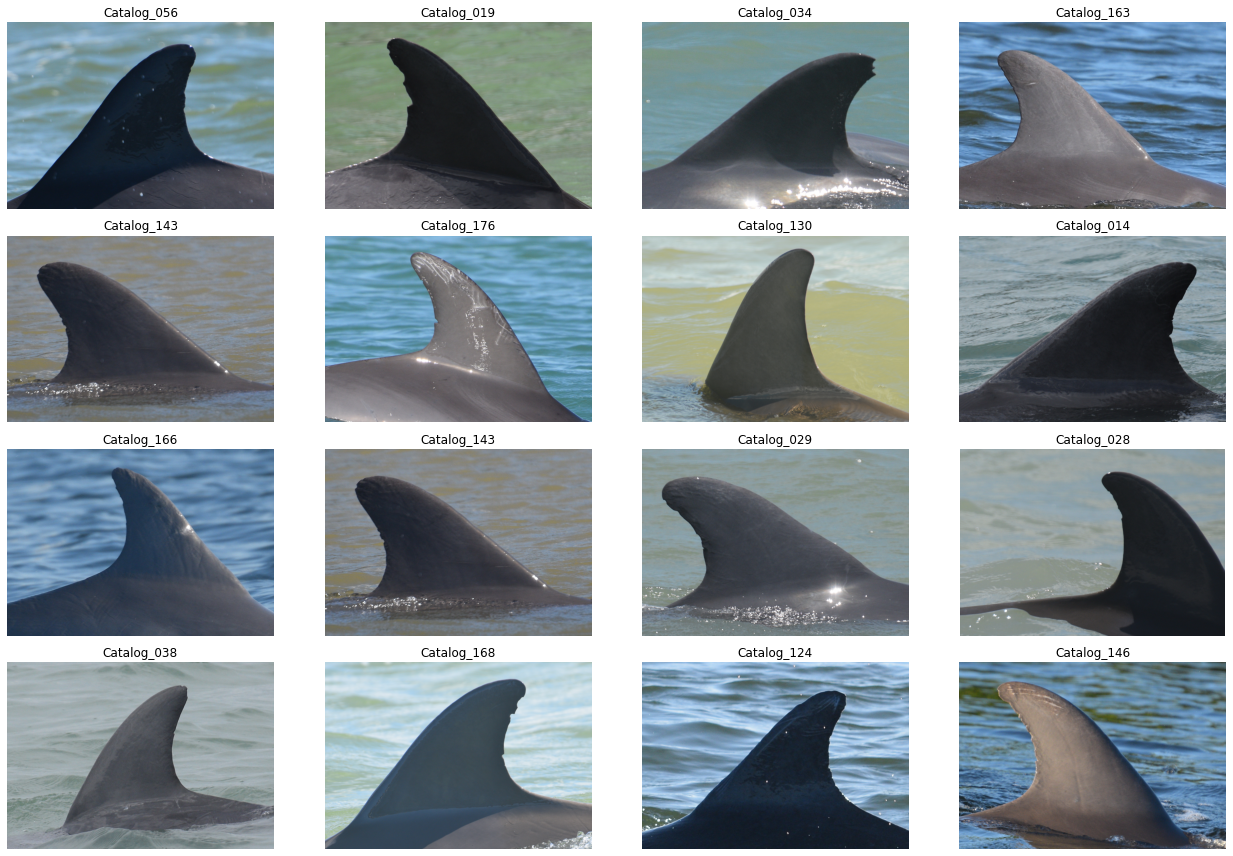
\includegraphics[scale=0.3]{Chapter6/figs/SDRP_egs_tiled.png}
	\end{center}
	\caption{Example images from the SDRP dataset with filenames displayed.}
	\label{fig:sdrp-example}
\end{figure}

The SDRP data was provided pre-split with 200 images, each of a unique individual, acting as the existing photo-id catalogue and the remaining 50 serving as images captured during a given day's fieldwork. Each image in the encounter set also contained a single individual however some individuals were captured multiple times. As such, there was a 23 individual overlap between the catalogue and encounter sets. 

To generate a train-test split capable of training an SNN, the catalogue set was reduced down to contain only the 23 individuals contained within the encounter set. Once filtered, both sets of images were ran through the Mask R-CNN dorsal fin detector and post processed using the methodology outlined in Section \ref{ch:cetDet,sec:postProcessing}. No images in this data had been seen by the detector, either during training or previous evaluation. Once generated, a \texttt{noise} class was manually created which contained all erroneously detected mask components. As the detector failed to accurately detect individual \texttt{19}, all components were marked as \texttt{noise}, resulting in a 23 class dataset. In cases where the detector had mistakenly detected the same fin twice, provided the two masks were not identical then both masks were kept - analogous to offline data augmentation. An example of this can be seen in Figure \ref{fig:sdrp-double-mask-eg}.

\begin{figure}
	\begin{center}
		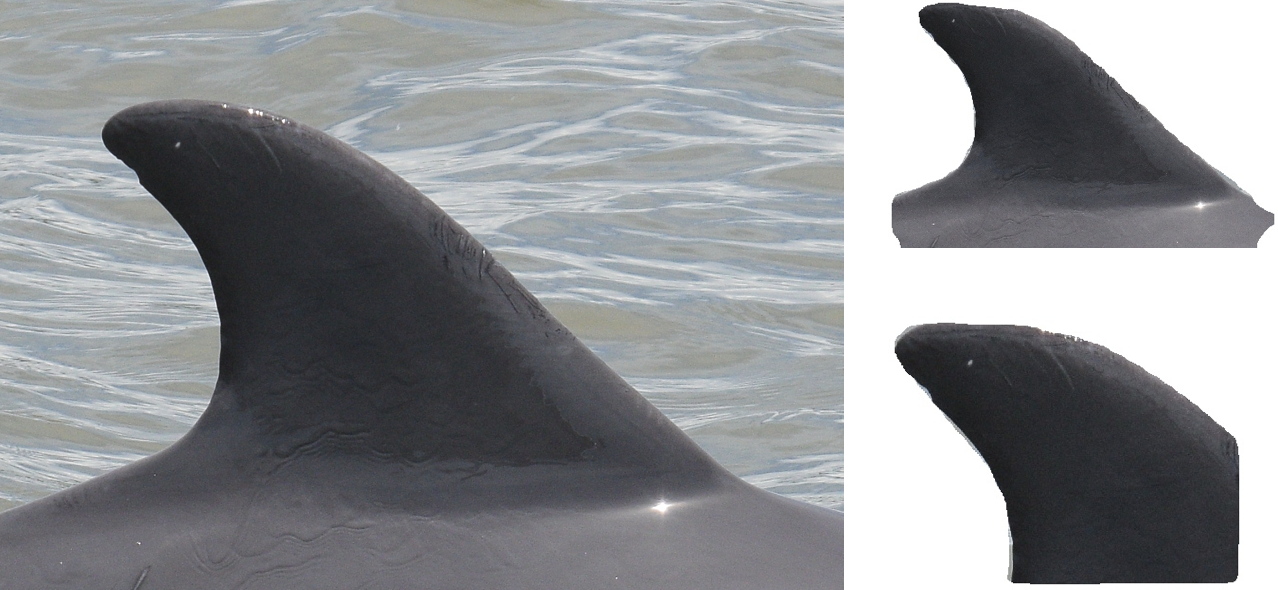
\includegraphics[scale=0.5]{Chapter6/figs/SDRP-double-mask-eg-indv-13.png}
	\end{center}
	\caption{Left: Image of individual \texttt{13} from the original SDRP catalogue set. Right: Example masks generated for the Left image. Both masks are kept for use in training as they were deemed to be sufficiently different.}
	\label{fig:sdrp-double-mask-eg}
\end{figure}

After detection and processing the resultant SDRP dataset contained a total of 123 images, significantly smaller than the NDD AU SMRU dataset which was used to evaluate the SNN-based approach previously. Retaining the split provided by the SDRP whereby the train set was generated from the catalogue and the test set from the encounter leads to a 35-65 train-test split, an inversion of what would be expected when training machine learning models. The class distribution for the SDRP dataset can be seen in Figure \ref{fig:sdrp-dist}. As like with the NDD AU SMRU dataset, the \texttt{noise} class is once again dominant. A colour threshold of 50\% was again utilised during post-processing with no correct detections erroneously discarded, suggesting this is an acceptable general value.

\begin{figure}[h]
	\begin{center}
		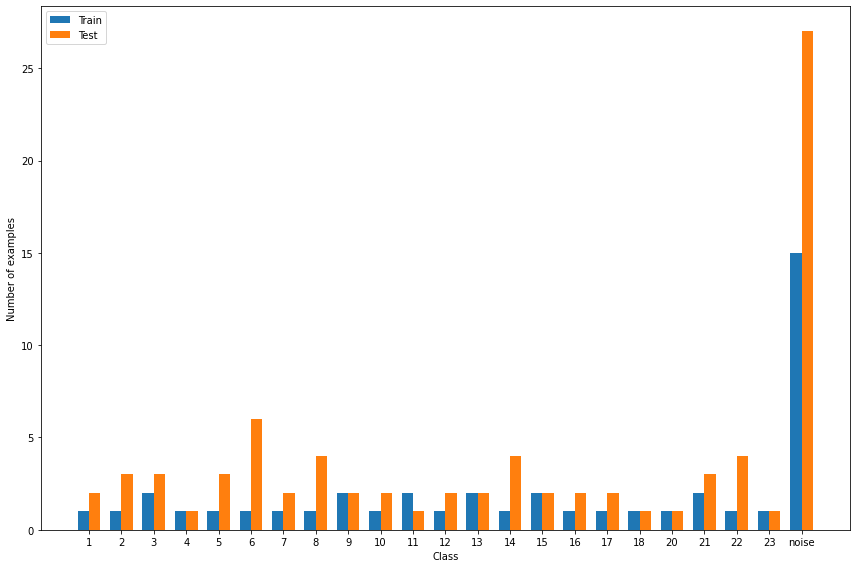
\includegraphics[scale=0.38]{Chapter6/figs/SDRP-class-dist.png}
	\end{center}
	\caption{The class distribution for the SDRP dataset, split by set.}
	\label{fig:sdrp-dist}
\end{figure}

These properties lead to the SDRP dataset being extremely challenging for an SNN to train on. However it is also an accurate representation of what a real life photo-id catalogue dataset would look like in the initial stages of a survey, providing an excellent test of both the robustness and generalisability of the SNN-based approach to automatic most likely catalogue matching when only small amounts of training data are available. 

\section{Evaluation Using the SDRP Dataset}\label{ch:SNNGeneralisation,sec:SNNEvalWithSDRP}

Due to the small amount of data, it was not possible to create a meaningfully large and diverse validation set for the SDRP dataset. This prevented hyperparameter optimisation, and as such the decision was made to utilise the optimal hyperparameters located for the best performing SNN on the NDD AU SMRU dataset, alongside the same backbone architectures and data augmentation strategies defined in Section \ref{ch:ID,sec:SNNDevelopment}.

\begin{figure}[h]
	\begin{center}
		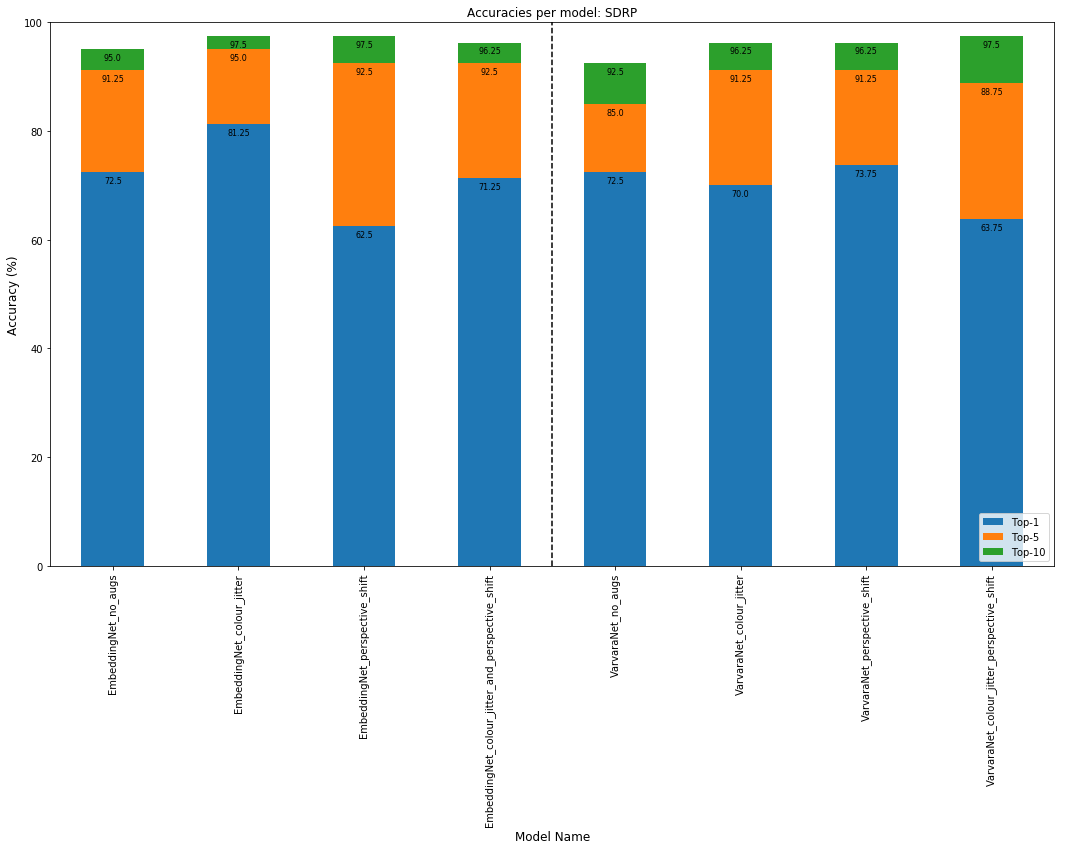
\includegraphics[scale=0.4]{Chapter6/figs/SDRP-normal-split-model-comparison.png}
	\end{center}
	\caption{Results of SNN training for the task of most likely catalogue matching on the SDRP dataset.}
	\label{fig:SDRP-normal-split-model-comparison}
\end{figure}

The results of model training on the SDRP dataset can be seen in Figure \ref{fig:SDRP-normal-split-model-comparison}, with each model evaluated using top-1, top-5, and top-10 accuracies.
Higher scores were achieved across the board on the SDRP dataset compared to the NDD AU SMRU dataset even without hyperparameter optimisation, however it is important to remember the smaller number of possible classes for the model to choose from which may inflate relative model performance.

Unlike training on the NDD AU SMRU data where best results were achieved without any augmentation, here the results are more mixed. Whilst the best top-10 accuracy, 97.5\%, is obtained using Colour Jitter and Perspective Shift augmentations (both together and separately), the best top-5 and top-1 accuracies were obtained using Colour Jitter only. These findings suggest that data augmentation strategy may be catalogue dependant and have a large impact on final model performance. 

Variation in backbone architecture had little effect on overall model performance. Interestingly models trained using a VarvaraNet backbone were more consistent, with a 10.00\% difference between the best and worst performing model, compared to an 18.75\% difference between those trained using an EmbeddingNet backbone. Overall however, the best performing model was determined to be an SNN using an EmbeddingNet backbone architecture and Colour Jitter data augmentation, which achieved 81.25\% top-1, 95.00\% top-5, and 97.50\% top-10 accuracies. This is in contrast to the best performing NDD AU SMRU model, made up of a VarvaraNet backbone architecture without any data augmentation. Using the optimal NDD AU SMRU model setup achieved 72.50\% top-1, 85.00\% top-5, and 92.50\% top-10 accuracies on the SDRP dataset. The use of an EmbeddingNet backbone as optimal for this dataset suggests that a simpler model structure may be best when working with smaller catalogues.

\subsection{SDRP Uncatalogued Individual Thresholding}\label{ch:SNNGeneralisation,sec:SNNEvalWithSDRP,sec:uncatalogued}

Evaluation of the best performing SDRP model's ability to flag uncatalogued individuals was undertaken. Unlike the model trained on the NDD AU SMRU dataset, a write-up of which is provided in Section \ref{ch:ID,sec:ModelSelection}, when trained on the SDRP dataset embedded images are placed closer together in the latent space. This means that the threshold values utilised for uncatalogued individual detection using prototype distance measurement and K-Nearest Neighbours (KNN) required modification to accurately output the necessary warnings. 

Experimentation outlined in Section \ref{ch:ID,sec:ModelSelection,subsec:UncataloguedIndividualThresholding,subsub:prototypes} determined it was possible to flag potentially uncatalogued individuals by checking the distance between an embedded image and its closest prototype. For the NDD AU SMRU dataset, the distance between an embedded image and its closest class prototype must be over 4.0 before a warning is displayed. Analysis of the distances between SDRP image embeddings and class prototypes however determined that this value was too large, whereby warnings were not displayed for some individuals who were uncatalogued. Through examination of the distances between each image and the generated prototypes, a threshold of 0.15 was determined to be optimal for the SDRP dataset, as it was small enough to trigger a warning for uncatalogued individuals whilst being large enough to not trigger in error when catalogued individuals were processed.


Discussion outlined in Section \ref{ch:ID,sec:ModelSelection,subsec:UncataloguedIndividualThresholding,subsub:KNN} showed that KNN could also be utilised for uncatalogued individual warning generation. Rather than measuring distances between embeddings like with prototype thresholding, here warnings are generated by calculating an uncertainty score based on the class labels of the $K$ nearest embeddings. When processing the NDD AU SMRU dataset it was determined that setting $K$ to 10 was sufficient, producing a warning when no single class made up 30\% or less of the nearest class labels. 

For the SDRP dataset, whilst an uncertainty of 30\% was found to be sufficient for generating a warning, setting $K$ to 10 was deemed too high. Utilising this value of $K$ resulted in some catalogued individuals incorrectly producing a warning, as a result of the compact nature of the embeddings in the SDRP latent space compared to that of the NDD AU SMRU space. Evaluation of each test image's neighbour in the latent space determined that setting $K = 5$ was optimal. Using this value ensured that warnings were displayed when uncatalogued individuals were processed, but prevented warning generation when processing examples of individuals present during training. 

\begin{figure}
	\begin{center}
		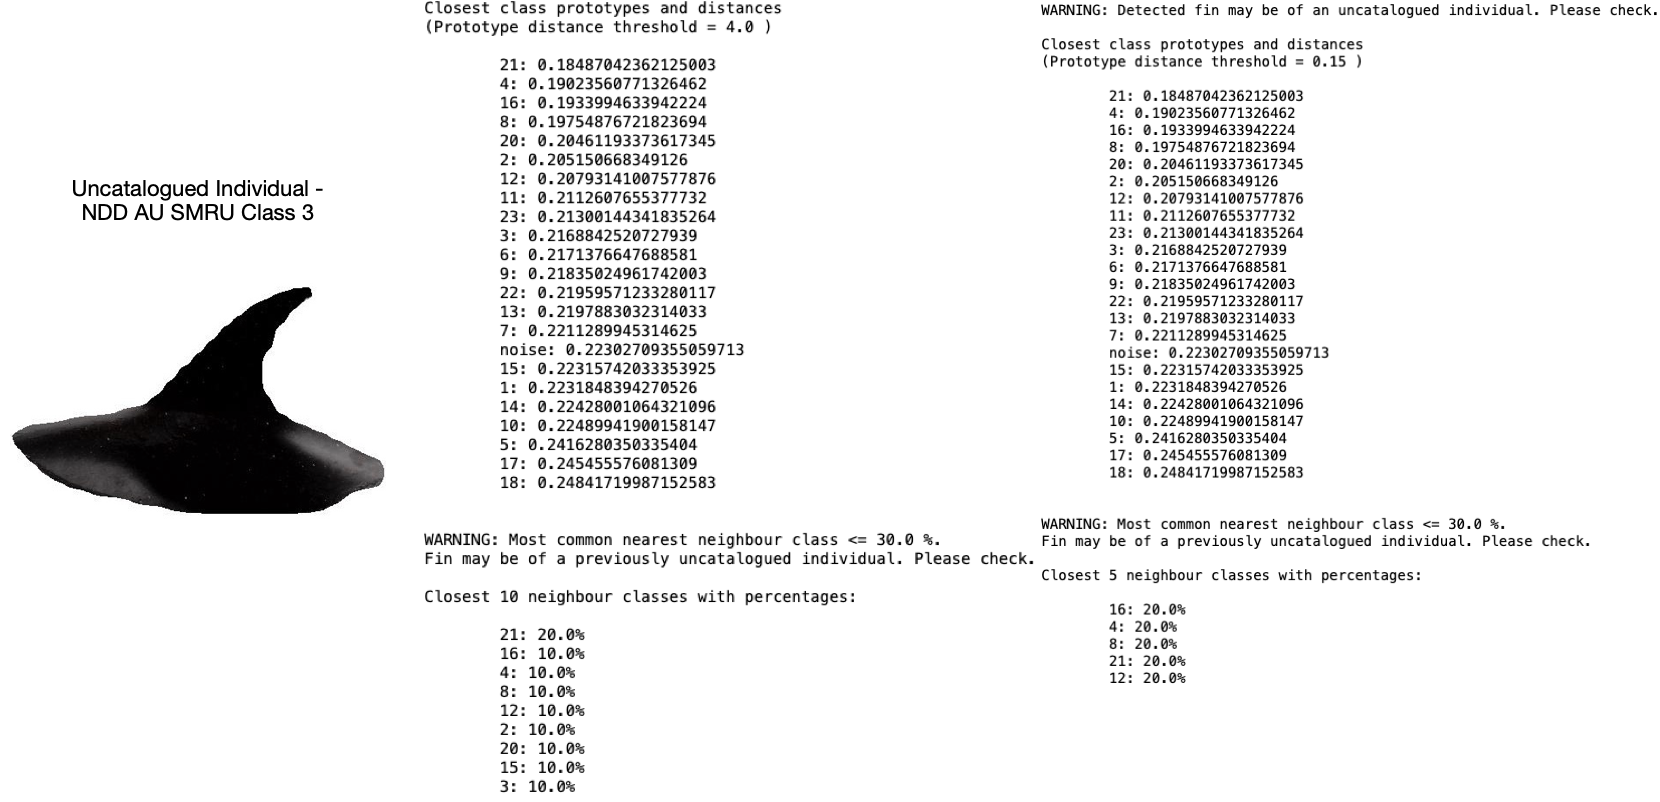
\includegraphics[scale=0.5]{Chapter6/figs/uncatalogued-individual-thresholding.png}
	\end{center}
	\caption{Example uncatalogued individual thresholding for the SDRP dataset using an individual not present during training (image taken from the NDD AU SMRU dataset). The resultant Euclidean distances between the input image's embedding and the existing class prototypes are shown. No warning has been generated when the minimum distance threshold is set to 4.0, however one has been when the threshold is set to 0.15. Uncertainty scores generated using K-Nearest Neighbours clustering are also shown. Warnings have been displayed both when $K = 10$ and $K = 5$ using an uncertainty threshold of 30\%.}
	\label{fig:uncatalogued-individual-example-sdrp}
\end{figure}

Example warning generation using both prototype distance measurement and KNN for an uncatalogued individual can be seen in Figure \ref{fig:uncatalogued-individual-example-sdrp}. Here, an example from the NDD AU SMRU dataset has been processed by the SNN trained on the SDRP dataset, and so warnings should be generated both by prototype distance measurement and KNN. As can be seen, when utilising a minimum prototype distance of 4.0 no warning is generated. Changing this value to 0.15 however ensures a warning is generated. When checking using KNN, warnings are produced both when $K$ is set to 10 and 5.

Figure \ref{fig:catalogued-individual-example-sdrp} shows example warning generation for an individual present during SNN training on the SDRP dataset. 

%%% Noise thresholding is fine with both prototypes and KNN



\begin{figure}
	\begin{center}
		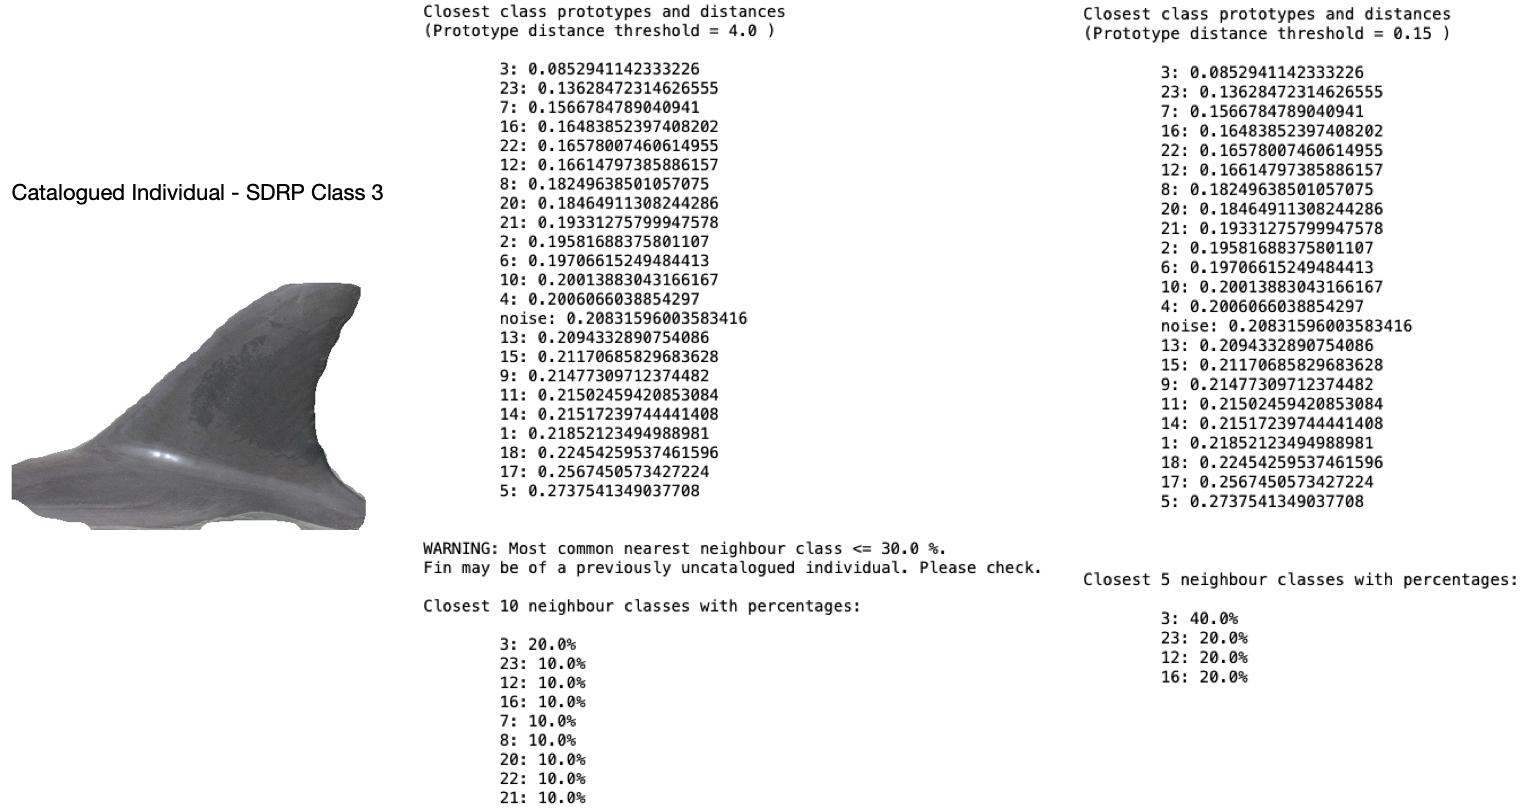
\includegraphics[scale=0.5]{Chapter6/figs/catalogued-individual-thresholding.png}
	\end{center}
	\caption{Example uncatalogued individual thresholding for the SDRP dataset using an individual present during training. The resultant Euclidean distances between the input image's embedding and the existing class prototypes are shown. No warning have been generated when the minimum distance threshold is set to either 4.0 or 0.15. Uncertainty scores generated using K-Nearest Neighbours clustering are also shown. A warning is displayed when $K = 10$ but not when $K = 5$, with both using an uncertainty threshold of 30\%.}
	\label{fig:catalogued-individual-example-sdrp}
\end{figure}






% Unseen individual thresholding:
% Struggles with the SDRP dataset
%% The latent space created for the dataset is smaller than the one for NDD AU SMRU, leading to prototypes being closer together
%% Suggest that thresholds are catalogue dependant and may need to be tuned when a new model is created /retrained
% Using individual only for uncatalogued individual



\subsection{Effect of Training Set Size on Model Backbone Selection}\label{ch:SNNGeneralisation,sec:SNNEvalWithSDRP,sec:reversedSDRP}

 As previously mentioned, the SDRP catalogue was provided pre-divided which, once post-processed, produced a 35-65 train-test split. As this training set is much smaller than what would normally be expected for developing a deep learning model, experimentation was undertaken to evaluate the hypothesis that a simpler model structure is best when low volumes of catalogue data is available during training. To this end, the dataset splits were reversed such that the test set was used for model training and the train set was used for evaluation. For consistency, the same model backbones and data augmentation strategies were utilised during training, as were the optimal NDD AU SMRU hyperparameters. 

 \begin{figure}
 	\begin{center}
 		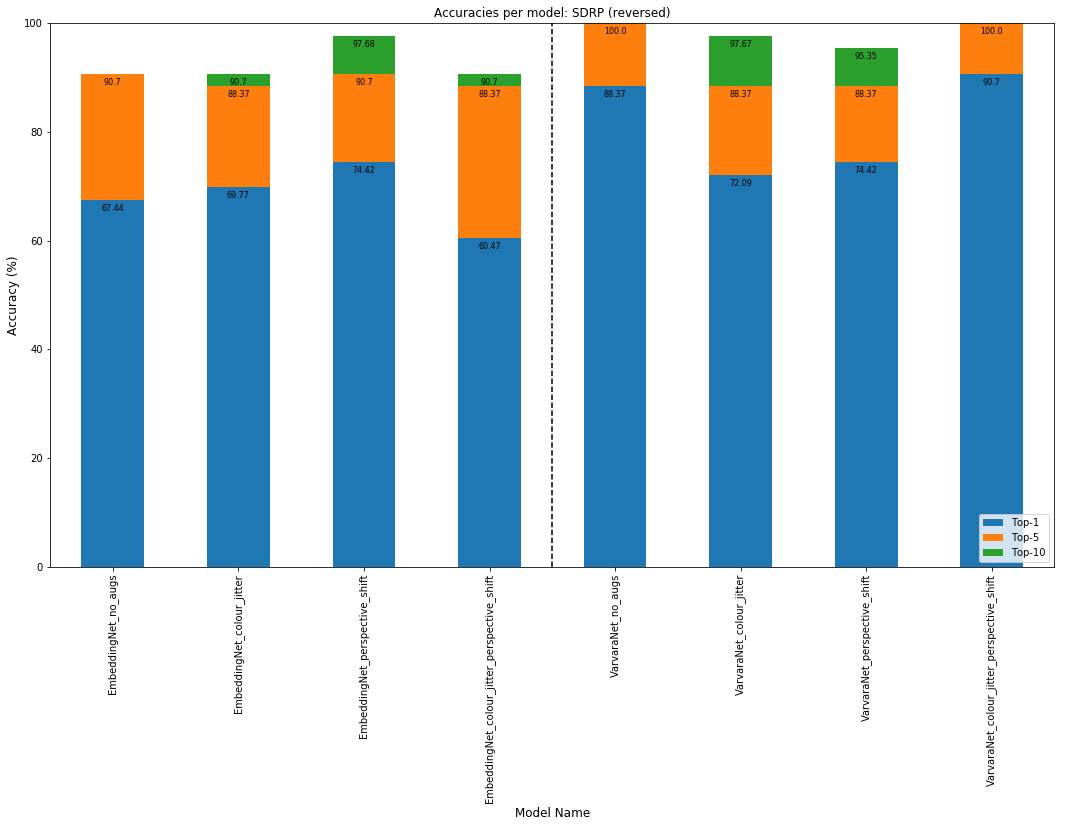
\includegraphics[scale=0.4]{Chapter6/figs/SDRP-reversed-split-model-comparison.png}
 	\end{center}
 	\caption{Results of SNN training for the task of most likely catalogue matching on the reversed SDRP dataset.}
 	\label{fig:SDRP-reversed-split-model-comparison}
 \end{figure}

The top-1, top-5, and top-10 accuracies for the trained models can be seen in Figure \ref{fig:SDRP-reversed-split-model-comparison}. By reversing the train-test split, a drop in performance is observed for all bar one of the models trained using an EmbeddingNet backbone. For the single model where performance improves, increases of  11.92\% top-1 and 0.18\%  top-10 accuracies are observed, however a drop of 1.80\% top-5 accuracy is also seen. For those models trained using a VarvaraNet backbone increases in performance are observed for all models, with only two reporting slight drops in top-5 accuracy. 

In general, it can be observed that the increase in training data has lead to an overall performance boost for models trained using a VarvaraNet backbone whilst those with an EmbeddingNet backbone observe a performance drop. As such, the best performing model for the reversed split SDRP dataset now makes use of a VarvaraNet backbone alongside both Colour Jitter and Perspective Shift data augmentation strategies. This supports the hypothesis that backbone architecture selection is influenced by the size of the initial training set, and that more complex models are required to fully capture the fine-grain nature of larger photo-id catalogues. These findings also provide further evidence to support the idea that data augmentation strategies are catalogue dependant. 

It should be noted however that the best performing model achieves 100\% top-5 and top-10 accuracies, suggesting the possibility of model overfitting. Whilst the model may be capable of always providing a match within the first five results, this is likely a product of dataset size causing an inflation in model performance. It is expected that these accuracies would decrease when utilising more data quantity, either through an increase in the number of classes or examples per class, as this would provide an increase in data variation.







% Section looking at effect of AU SMRU on the models (Effect of AU SMRU on Model notebook)
% Section looking at effect of background noise retention (may need to rename chapter?)

% Conclusion




